\documentclass{beamer}
%
% Choose how your presentation looks.
%
% For more themes, color themes and font themes, see:
% http://deic.uab.es/~iblanes/beamer_gallery/index_by_theme.html
%
\mode<presentation>
{
  \usetheme{Boadilla}      % or try Darmstadt, Madrid, Warsaw, ...
  \usecolortheme{beaver} % or try albatross, beaver, crane, ...
  \usefonttheme{default}  % or try serif, structurebold, ...
  \setbeamertemplate{navigation symbols}{}
  \setbeamertemplate{caption}[numbered]
  
} 

\usepackage{xcolor,colortbl}
\usepackage[english]{babel}
\usepackage[utf8x]{inputenc}
\usepackage{courier}
\usepackage{dsfont}
\usepackage{verbatim} 
\usepackage{enumerate}
\usepackage{tikz}
\usepackage{multirow}
\usepackage{bbm}
\usepackage{amsmath}
\usepackage{venndiagram}
\usepackage{epigraph} 
%\usepackage{xcolor}



\usepackage{hyperref}
\hypersetup{
    colorlinks=true,
    linkcolor=blue,
    filecolor=magenta,      
    urlcolor=cyan,
}

% R stuff!
\usepackage{listings}
\definecolor{codegreen}{rgb}{0,0.6,0}
\definecolor{codegray}{rgb}{0.5,0.5,0.5}
\definecolor{codepurple}{rgb}{0.58,0,0.82}
\definecolor{backcolour}{rgb}{0.95,0.95,0.92}

\lstdefinestyle{mystyle}{
    backgroundcolor=\color{backcolour},    
    commentstyle=\color{codegreen},
    keywordstyle=\color{black},
    numberstyle=\tiny\color{codegray},
    stringstyle=\color{codepurple},
    basicstyle=\ttfamily\footnotesize,
    breakatwhitespace=false,         
    breaklines=true,                 
    captionpos=b,                    
    keepspaces=true,                 
    numbers=left,                    
    numbersep=5pt,                  
    showspaces=false,                
    showstringspaces=false,
    showtabs=false,                  
    tabsize=2
}

\lstset{style=mystyle}



%% Size options for nested itemized lists
\usepackage{relsize}
\setbeamerfont{itemize/enumerate body}{parent=normal text}
\setbeamerfont{itemize/enumerate subbody}{parent=normal text,size=\relsize{-1}}
%\setbeamerfont{itemize/enumerate subsubbody}{parent=normal text,size=\relsize{-1}}




\setbeamertemplate{enumerate items}[default]
\setbeamertemplate{itemize item}[triangle]

%\setitemize{label=\usebeamerfont*{itemize item}%
%  \usebeamercolor[fg]{itemize item}
%  \usebeamertemplate{itemize item}}


\usetikzlibrary{shapes,decorations,arrows,calc,arrows.meta,fit,positioning}
\tikzset{
    -Latex,auto,node distance =1 cm and 1 cm,semithick,
    state/.style ={ellipse, draw, minimum width = 0.7 cm},
    point/.style = {circle, draw, inner sep=0.04cm,fill,node contents={}},
    bidirected/.style={Latex-Latex,dashed},
    el/.style = {inner sep=2pt, align=left, sloped}
}

\newcommand{\Mypm}{\mathbin{\tikz [x=1.4ex,y=1.4ex,line width=.1ex] \draw (0.0,0) -- (1.0,0) (0.5,0.08) -- (0.5,0.92) (0.0,0.5) -- (1.0,0.5);}}%



%% For block quote
\usepackage{etoolbox}
\AtBeginEnvironment{quote}{\par\singlespacing\small}


\title[STA 209]{Regression Error}
\subtitle{}
%\author{}
\author{Grinnell College}
\date{December 9, 2024}

\graphicspath{{img/}}

\begin{document}

\begin{frame}
  \titlepage
\end{frame}

\begin{frame}{Review}

\begin{itemize}
\item Regression models a linear relationship between response variable $y$ and explanatory variable $X$ of the form
\begin{align*}
y = \beta_0 + \beta_1 X + \epsilon
\end{align*}
\item Can expand this to include combinations of explanatory variables (quant. and cat.)
\end{itemize}

\end{frame}

\begin{frame}{Error Terms}

\begin{align*}
y = \beta_0 + X \beta_1 + \epsilon 
\end{align*} \vspace{4mm}

Assumptions:
\begin{itemize}
\item Linear relationship between X and y
\item Error term is normally distributed, $\epsilon \sim N(0, \sigma)$
\item Error should be the same for all values of $X$, i.e., error same for all observations
\end{itemize} \vspace{4mm}

Analyzing the error terms gives us a way to test the assumptions of our model

\end{frame}


\begin{frame}{Residuals}
Visually, let's review what residuals look like
\begin{itemize}
    \item residuals represent how far off our prediction is
\end{itemize}
\begin{center}
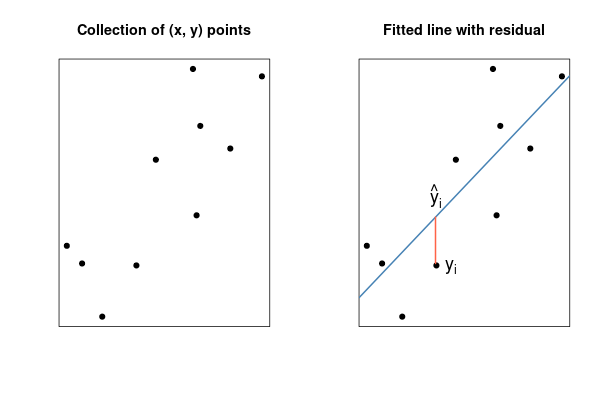
\includegraphics[scale=0.5]{error.png}
\end{center}
\end{frame}



\begin{frame}
\begin{center}
Part 1: Checking Assumptions
\end{center}
\end{frame}

\begin{frame}{Residuals and assumptions}
\begin{columns}

  \begin{column}{0.45\textwidth}
  Three common ways to investigate residuals visually:
  \begin{enumerate}
  \item Plot histogram of residuals (normality)
  \item Plot residuals against covariate (linear trend, changing variance)
  \item Plot residuals against new covariates (pattern identification)
  \end{enumerate}
  \end{column}
  \begin{column}{0.45\textwidth}
\begin{center}
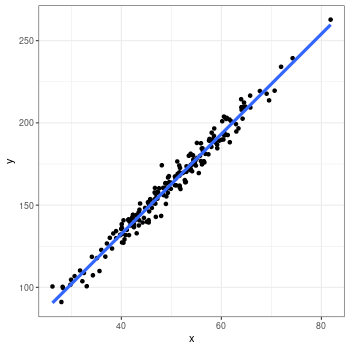
\includegraphics[scale=0.45]{norm_fit.png}
\end{center}
  \end{column}

\end{columns}
\end{frame}

\begin{frame}{Checking Normality}
Histogram of Residuals should be $\approx$Normal if our model is doing well \vspace{2mm}

Residuals should not have a pattern other than 'blob of points' in a Resid. vs. Expl. Var. plot
\begin{center}
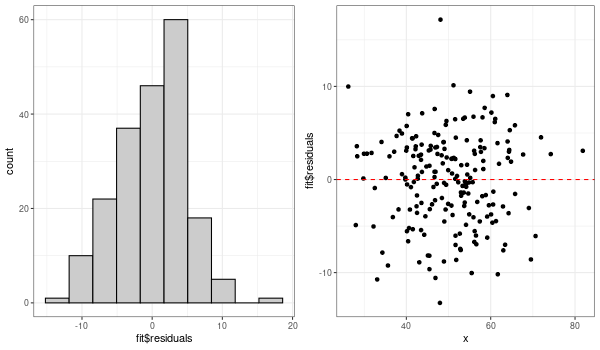
\includegraphics[scale=0.5]{norm_errors.png}
\end{center}
\end{frame}

\begin{frame}{Tests of linearity}
Residual vs. Explanatory plot makes seeing non-linearity easier
\begin{center}
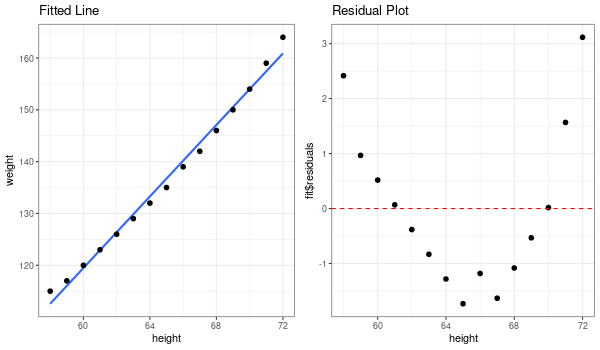
\includegraphics[scale=0.5]{women_error.png}
\end{center}
\footnotesize
\begin{itemize}
    \item linear regression could still be useful!
    \item but we could also look at doing something more complicated if we really cared
\end{itemize}
\end{frame}

\begin{frame}{Tests of linearity}
\small
Sometimes a transformation of a variable can help correct trends ($\log (\text{weight})$)
\begin{center}
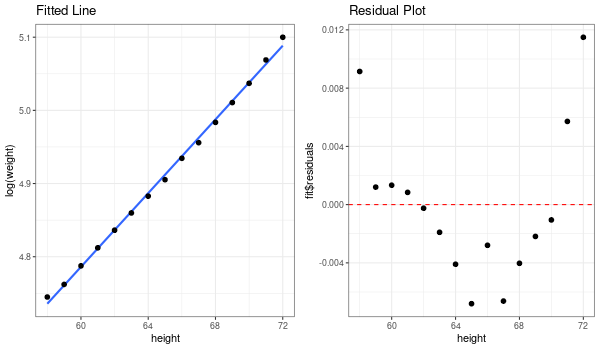
\includegraphics[scale=0.5]{women_error_log.png}
\end{center}
\end{frame}

\begin{frame}{Heteroscedasticity}
\small
Hetero = different, scedastic = random
\begin{center}
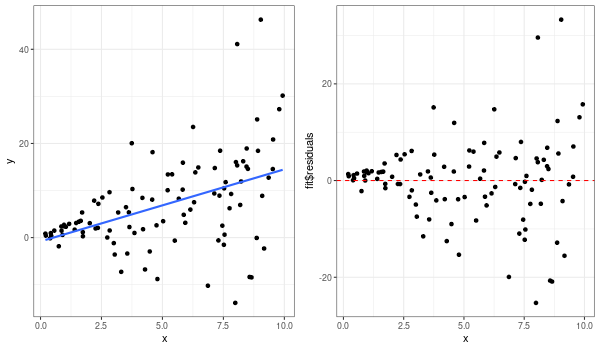
\includegraphics[scale=0.5]{non_homog.png}
\end{center}
\end{frame}




\begin{frame}
\begin{center}
Part 2: Investigating Patterns
\end{center}
\end{frame}

\begin{frame}{Considering new covariates}


\begin{columns}

  \begin{column}{0.45\textwidth}
  Suppose I have:
  \begin{itemize}
  \item Quantitative outcome $y$
  \item Quantitative predictor $X$
  \item Categorical predictor $gp$
  \end{itemize}
  \end{column}
  \begin{column}{0.45\textwidth}
\begin{center}
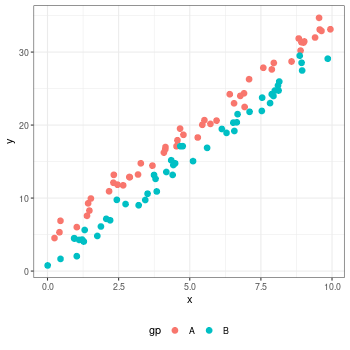
\includegraphics[scale=0.45]{color_cat.png}
\end{center}
  \end{column}

\end{columns}

\end{frame}

\begin{frame}{Considering new covariates}
\begin{center}
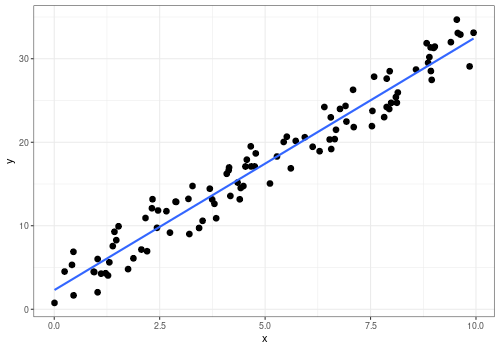
\includegraphics[scale=0.5]{miss_cat.png}
\end{center}
\end{frame}

\begin{frame}{Considering new covariates}
\begin{center}
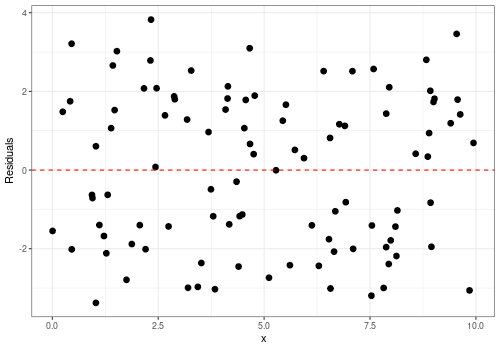
\includegraphics[scale=0.5]{miss_cat_res.png}
\end{center}
\end{frame}


\begin{frame}{Considering new covariates}
\begin{center}
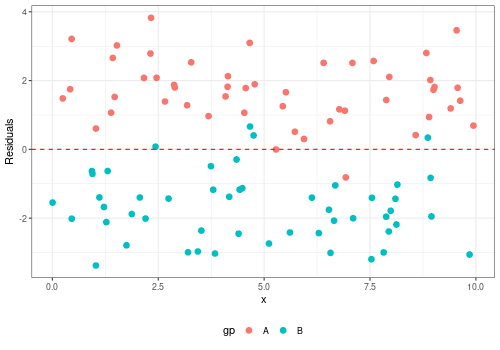
\includegraphics[scale=0.5]{miss_cat_res2.png}
\end{center}
\end{frame}

\begin{frame}{Considering new covariates}
\begin{center}
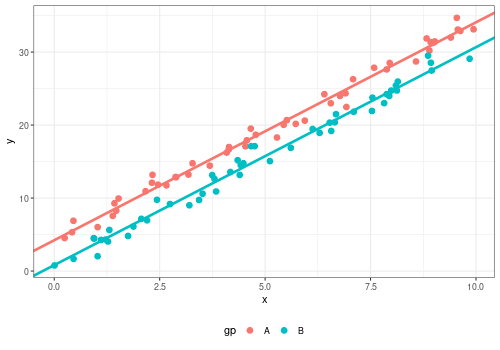
\includegraphics[scale=0.5]{have_cat.png}
\end{center}
\end{frame}


\begin{frame}{Considering new covariates}
these residuals are from the model that \textit{also} includes the gp variable
\begin{center}
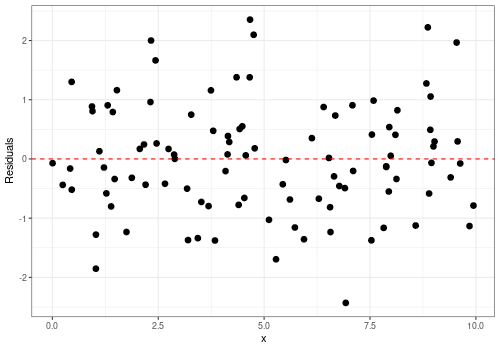
\includegraphics[scale=0.5]{have_cat1.png}
\end{center}
\end{frame}


\begin{frame}{Considering new covariates}
if we color by 'gp' we see that the pattern is now random about 0
\begin{center}
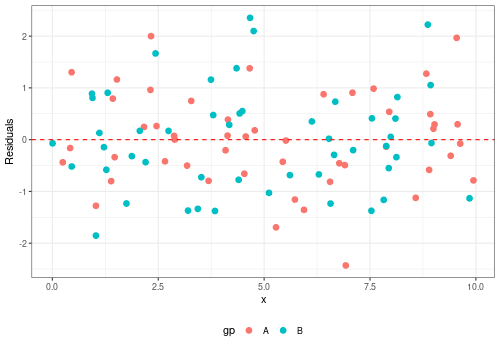
\includegraphics[scale=0.5]{have_cat2.png}
\end{center}
\end{frame}


\begin{frame}{Correlated Covariates}
Consider a simple linear model in which a covariate $X$ is used to predict some value $y$

\begin{align*}
\hat{y} = \hat{\beta}_0 + X \hat{\beta}_1 
\end{align*}

The residuals associated with this describe the amount of variability that \textit{is yet to be explained}
\begin{align*}
e = y - \hat{y}
\end{align*}
The idea is to find new covariates \textit{associated} with this residual, in effect ``mopping up" the remaining uncertainty
\end{frame}


\begin{frame}{Considering new covariates}

Last week (Friday) we considered an example predicting vehicle fuel economy (mpg) with three separate models:

\begin{enumerate}
\item Using weight
\item Using weight and engine displacement
\item Using weight and quarter mile time
\end{enumerate}


\end{frame}

\begin{frame}{Correlated Covariates}
Let's say I have a regression using wt to predict mpg. We are looking for a new variable to add to the model. Which of these would be better to use?
\begin{center}
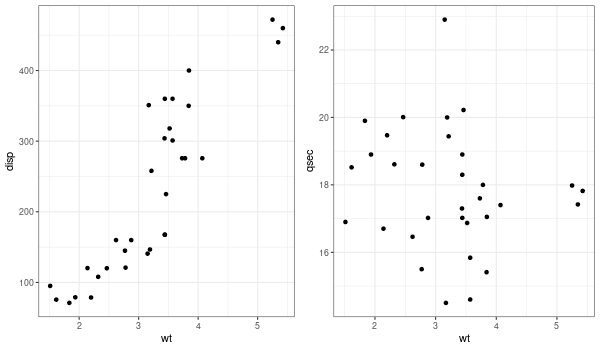
\includegraphics[scale=0.45]{cor_compare.png}
\end{center}
\small
\begin{itemize}
    \item because wt and disp are correlated, much of the info in disp is already contained within wt $\rightarrow$ probably not much improvement if we add it
\end{itemize}
\end{frame}

\begin{frame}[fragile]{Correlated Covariates}

\begin{lstlisting}[language=R,basicstyle=\ttfamily\scriptsize]
> lm(mpg ~ wt, mtcars) %>% summary()

            Estimate Std. Error t value     Pr(>|t|)    
(Intercept)   37.285      1.878   19.86   < 0.000002 ***
wt            -5.344      0.559   -9.56     0.000013 ***
R-squared = 0.75
\end{lstlisting}
\begin{lstlisting}
> lm(mpg ~ wt + disp, mtcars) %>% summary()

            Estimate Std. Error t value      Pr(>|t|)    
(Intercept) 34.96055    2.16454   16.15  0.000000049 ***
wt          -3.35083    1.16413   -2.8        0.0074 ** 
disp        -0.01772    0.00919   -1.93       0.0636 .  
R-squared = 0.78
\end{lstlisting}
\begin{lstlisting}
> lm(mpg ~ wt + qsec, mtcars) %>% summary()

            Estimate Std. Error t value       Pr(>|t|)    
(Intercept)   19.746      5.252    3.76        0.00077 ***
wt            -5.048      0.484  -10.43 0.000000000025 ***
qsec           0.929      0.265    3.51        0.00150 ** 
R-squared = 0.82
\end{lstlisting}
\end{frame}

\begin{frame}{Residual Plots}
\begin{center}
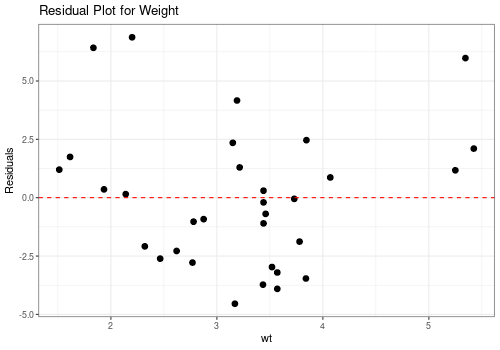
\includegraphics[scale=0.5]{wt_resid.png}
\end{center}
\end{frame}

\begin{frame}{Residual Plots}
\begin{center}
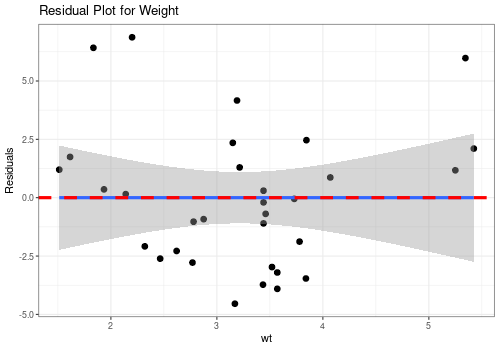
\includegraphics[scale=0.5]{wt_resid2.png}
\end{center}
\end{frame}

\begin{frame}{Residual Plots}
\begin{center}
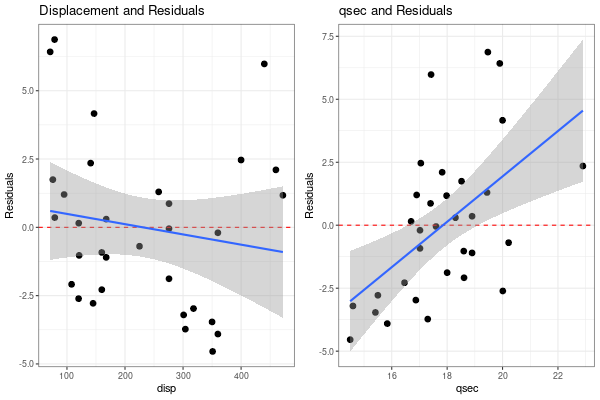
\includegraphics[scale=0.5]{mtcars_resid.png}
\end{center}
\end{frame}



\begin{frame}{Key Takeaways}
\begin{enumerate}
\item Number of assumptions for linear model
\begin{itemize}
\item Linearity 
\item Normal errors
\item Homoscedasticity
\end{itemize}
\item Need way to determine which new variables to add to model
\item Examining errors effective way to test assumptions and investigate new covariates
\end{enumerate}
\end{frame}

%\begin{frame}
%\begin{columns}
%
%  \begin{column}{0.45\textwidth}
%%
%  \end{column}
%  \begin{column}{0.45\textwidth}
%%
%  \end{column}
%
%\end{columns}
%\end{frame}


\end{document}
